\documentclass[a4paper,twoside,12pt,openright]{report}

%% Language %%%%%%%%%%%%%%%%%%%%%%%%%%%%%%%%%%%%%%%%%%%%%%%%%
\usepackage[francais]{babel}
\usepackage[utf8]{inputenc}
\usepackage[T1]{fontenc}
\usepackage{lmodern} 
\usepackage{hyperref}

%% Packages for Graphics & Figures %%%%%%%%%%%%%%%%%%%%%%%%%%
\usepackage{graphicx} 

%% Math Packages %%%%%%%%%%%%%%%%%%%%%%%%%%%%%%%%%%%%%%%%%%%%
\usepackage{amsmath}
\usepackage{amsthm}
\usepackage{amsfonts}
\usepackage{fullpage}
%%%%%%%%%%%%%%%%%%%%%%%%%%%%%%%%%%%%%%%%%%%%%%%%%%%%%%%%%%%%%
%% DOCUMENT
%%%%%%%%%%%%%%%%%%%%%%%%%%%%%%%%%%%%%%%%%%%%%%%%%%%%%%%%%%%%%
\begin{document}
\begin{titlepage}
	\centering
	\vspace{1cm}
	{\scshape\large Université Paris Nanterre \par}
	\vspace{1cm}
	
\includegraphics[width=0.25\textwidth]{univ.JPG}\par
	\vfill
	{\scshape\Huge Rapport de stage M1 MIAGE\par}
	\vspace{1cm}
	{\LARGE Auteur : Thibault Sartre\par}
	\vspace{1cm}
	{\Large Stage de Développeur\par}
	\vspace{1cm}
	{\large Avril à Juillet 2018\par}
	\vspace{1cm}
	\vfill
	{\large Tuteur académique:}
	{\large Emmanuel Hyon\par}
	\vspace{0.5cm}
	{\large Tuteur entreprise:}
	{\large Abdoullah Boufrine}
	\vfill
	\vfill
	\vfill
	
\includegraphics[width=0.15\textwidth]{orange.png}\par
	\vspace{1cm}
	{\large Entreprise Orange\par}


\end{titlepage}
\renewcommand{\contentsname}{Sommaire}
\tableofcontents{}
\newpage
\chapter{Introduction}
\section{Remerciements}
Trouver un stage de trois mois n'est pas facile. C'est pourquoi je remercie la société Orange de m'avoir accueilli à nouveau.\\
Merci à M Samy Damien, responsable du service 3MU, d'avoir accepté ma candidature et de m'avoir intégré à l'équipe.\\
Merci à l'ensemble des membres de l'équipe 3MU pour leur accueil et les conseils qu'ils ont pu me prodiguer au cours de ces trois mois.\\
Et je tiens à remercier plus particulièrement mon maître de stage M Abdoullah Boufrine, concepteur/développeur dans le service, qui m'a accompagné tout au long de cette expérience professionnelle en me faisant confiance et en étant disponible.\\
\section{Introduction}
Dans le cadre de mon Master MIAGE, je dois effectuer un stage d’une durée de trois mois minimum.\\
Dans le parcours MIAGE, le développement est ce qui me plait le plus.\\
Mon projet professionnel m'amène vers les métiers de la programmation.\\
C'est pourquoi j'ai cherché un stage qui répondrait à mes attentes, me permettrait d'utiliser mes acquis, découvrir de nouveaux langages de programmation et de nouvelles méthodes de travail.\\
En m'adressant à la société Orange j'étais certain de le trouver.\\
J'espérais pouvoir réaliser le(s) projet(s) de manière efficace tout en produisant un travail de qualité.\\
Je vais donc vous présenter la société Orange et ses secteurs d'activités puis vous présenter mes missions.\\
\chapter{Présentation}
\section{Entreprise}
Orange est une entreprise française de télécommunication.\\
C'est aussi une entreprise internationale qui est composée de 155 000 salariés dans le monde.\\
Elle possède 263 millions de clients dont 3,3 millions de clients fibre.\\
 Il y a 29 millions de clients d’Orange Money (transfert d'argent simplifié).\\ 
 Le réseau mobile 4G a été déployé dans 18 pays.\\
 Orange possède aussi 450 000 kms de câbles sous-marins.\\
Orange investit 732 millions d’euros pour la recherche et l’innovation.\\
Elle soutient 224 start-up dans le cadre du programme Orange Fab.\\
 Il s’agit de la 51ème marque mondiale en 2016.\\ 
 Elle dispose du meilleur réseau mobile en France pour la 6ème fois consécutive (classement Arcep).
\subsection{Unité : UI IDF Centre}
L'unité d'Intervention Île-de-France Centre (UI IDF Centre) assure l'installation, la mise en service et la maintenance de tous les produits et services pour les clients Grand Public (Particulier et Professionnel en dehors des clients Entreprise ) de Paris et des Hauts de Seine.\\
Cette unité dépend de la direction Orange Île-de-France (
\emph{cf annexe A Direction Orange Île-de-France}
).\\
Son périmètre d'intervention concerne l'ensemble des activités d'intervention client Grand Public, la partie terminale du réseau et le déploiement de la fibre, en vue d'améliorer la qualité de service des clients et développer le chiffre d'affaires.\\
\begin{center}
\includegraphics[height=10cm]{organisation.PNG}\\
\itshape Schémas des départements de l'UI IDF Centre.
\end{center}
\begin{center}
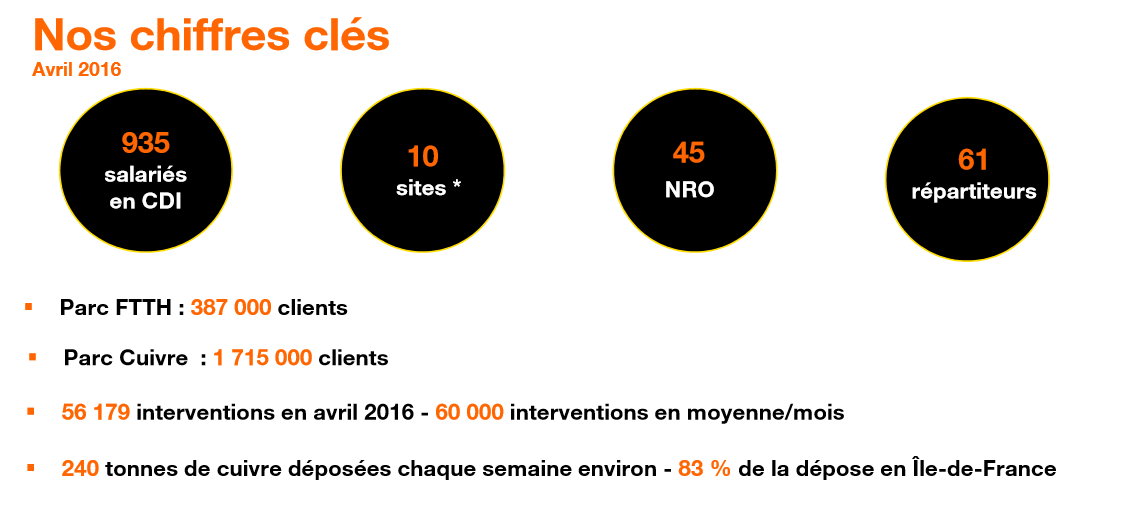
\includegraphics[height=8cm]{chiffre.PNG}\\
\itshape Chiffres clés du mois d'avril 2016 de l' UI IDF Centre.
\end{center}
\newpage
\subsection{Département : DEVRAP}
Développements Rapides (DevRap) est un département de l' UI IDF Centre.\\\\
DevRap a pour mission :
\begin{itemize}
\item Développer des solutions provisoires ou pérennes.
\item Offrir une réponse adaptée aux demandes urgentes.
\end{itemize}
Ce département est composé des équipes :
\begin{itemize}
\item Equipe Web et Peris managée par Claude Lapouge.
\item Equipe Celllule d'automatisation des tâches Opérationnelles (CATOP) managée par Philippe Bernard.
\item Equipe 3ème main de l'Utilisateur (3MU) managée par Samy Damien.
\end{itemize}
Chaque année tout le personnel du Département DevRap est invité à un séminaire.\\
Pendant ce séminaire un bilan est fait sur ce qui s'est passé durant l'année, un point est fait sur la stratégie future. Cette année une présentation tournera autour de la gouvernance adaptative.\\
Des activités et des jeux sont organisés. Le séminaire est donc un moment où l'on parle du passé et du futur tout en passant un bon moment en rencontrant tous les collègues. 
\subsection{Equipe d'accueil : 3MU}
\subsubsection{Description :}
Mon stage se déroule dans la structure Orange à DevRap du 09 avril 2018 au 06 juillet 2018, plus particulièrement dans l’équipe 3MU de la Direction de Solutions Paris.\\
Elle est composée d’un manageur ainsi que de 4 développeurs.\\\\
L’équipe 3MU développe des outils qui enchaînent à votre place les gestes répétitifs que vous réalisez plusieurs dizaines, voire centaines, de fois dans la journée.\\
Les travaux de l’équipe 3MU consistent à développer des scripts d’automatisation (automates) déclenchés sur demande. Ceux-ci évitent les imprécisions des saisies manuelles.\\
Ces automates sont mis à la disposition des utilisateurs finaux du SI d’Orange pour leur apporter confort, précision et efficacité.\\
3MU peut aussi ajouter de nouvelles fonctionnalités aux applications existantes.\\
L’équipe utilise principalement le logiciel Contextor basé sur du javascript, le langage AutoIt.\\
Pendant la période de mon stage ils ont commencé à avoir des formations pour utiliser un nouveau logiciel nommé NICE.\\

\subsubsection{Demande de projet à l'équipe}
\begin{center}
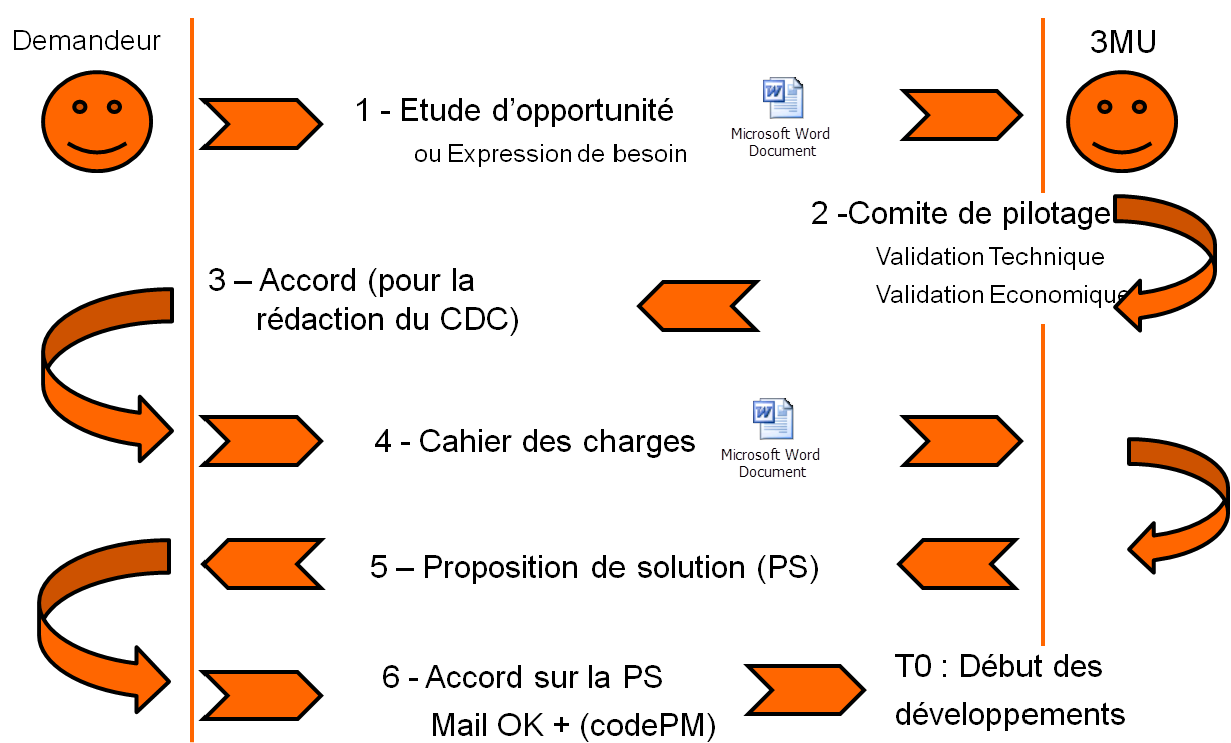
\includegraphics[height=10cm]{Demande_projet.PNG}\\
\itshape Schémas d'une demande de projet.
\end{center}
\vspace{1cm}
Etape 1 :	Le demandeur envoie une expression de besoin.\\\\
Etape 2 :	3MU  étudie l’expression de besoin et décide si  le projet est réalisable ou pas.\\\\
Etape 3 :	3MU envoie son accord pour la prise en charge du projet pour que le demandeur rédige un cahier des charges.\\\\
Etape 4 :	Le demandeur renvoie un cahier des charges.\\\\
Etape 5 :	3MU étudie le cahier des charges et envoie une Proposition de Solution.\\\\
Etape 6 :	Le demandeur envoie une réponse pour la Proposition de Solution.\\\\
Etape 7 :	Si la réponse reçue est positive, 3MU peut commencer le développement.
Le développement n’est lancé qu’à la fin car c’est un investissement qui nécessite des ressources humaines et financières et qui du coup doit être bien évalué et validé.
\newpage
%\subsection{Les réunions}
%\vspace{1cm}
\subsubsection{Réunions d'équipe}
Le manageur a mis en place une réunion d’équipe tous les mois ou plus si besoin.\\ 
Lors de ces réunions, chacun dit où il en est dans ses projets en cours (avancement, délai avant de terminer le projet, problèmes rencontrés) et présente les projets à venir (dates du début de développement, fonctionnalités).\\
Ceci permet un partage des connaissances, une montée en compétence de l'ensemble de l'équipe.\\
Lorsque de nouveaux projets arrivent, le chef d'équipe va alors les présenter aux membres de l'équipe pour décider qui va s'occuper de quel projet.\\
On peut échanger sur les sujets pour avoir l'avis des autres membres de l'équipe et éventuellement leur demander de l'aide. Par exemple lors d'une réunion, les membres de l'équipe ont pesé le pour et le contre du nouveau logiciel NICE qu'ils étaient en train de découvrir.
\subsubsection{Réunions téléphoniques}
J’ai participé à plusieurs réunions téléphoniques qui sont en rapport avec les projets que j'ai dû effectuer.\\ 
Dans ces réunions, les entités liées au projet sont présentes pour faire un point sur l’avancement de chacun. On vérifie si tout le monde possède une vision précise de ce qu’il doit faire.\\
Ces réunions permettent de se mettre d’accord sur ce qui est attendu.\\ 
Elles sont primordiales pour ne pas perdre de temps et pouvoir, au final, livrer dans les délais prévus.\\\\
Les réunions suivantes sont hebdomadaires pour permettre à l’équipe d’avancer en coordination avec l’acteur qui a sollicité notre aide afin de s’assurer que la qualification du besoin des utilisateurs est correcte et que nous sommes toujours bien en phase.\\\\
Certaines sont plus techniques. Dans ce dernier cas les réunions se font en petit comité où l'on parle plus précisément de ce qui est attendu.\\
Par exemple, quand on a reçu le projet "RMM", on devait prendre en main une application déjà existante (RMM). On a donc eu une réunion avec un développeur de l’application pour qu’il nous présente toutes ses fonctionnalités et qu'il nous présente grossièrement les évolutions à faire.\\ 
\newpage
\chapter{Compétences techniques acquises}
%\section{Langage Javascript}
%L'utilisation du logiciel Contextor nécessite la connaissance du langage Javascript.\\
%Sur les conseils de mon tuteur, j’ai appris les bases du langage Javascript en quelque jours sur internet pour pouvoir utiliser le logiciel Contextor et ainsi enrichir mes connaissances.
%\section{Langage AutoIt}
%J’ai dû apprendre les bases du langage AutoIt pour pouvoir modifier l'application "MacPeb" et réaliser des recherches d'éléments sur une page Web, ces deux sujets sont détaillés dans le chapitre missions effectuées.\\ 
%Ce langage permet la création d’automates de la même manière que Contextor. 
%\section{Logiciel Wordpress}
%J’ai appris à utiliser le logiciel Wordpress pour la mise à jour du blog de l'équipe\\
%Ce logiciel permet la création et la gestion de sites internet d'une manière facilitée.\\
%Il permet de créer un site complet sans écrire une seule page html à la main.
%\newpage
\section{Logiciel Contextor}
\subsection{Les avantages}
J’ai appris à utiliser le logiciel Contextor pour réaliser un projet.\\\\ 
Ce logiciel récupère les entrées/sorties et analyse les évènements survenant sur le poste de travail du salarié.\\
En parallèle, Contextor suit un script Javascript qui va déclencher des actions sur le poste de travail, par exemple copier un champ pour le coller dans un autre, cliquer sur des boutons, manipuler des pages web.\\\\
Il permet donc de capturer des images de page web pour ensuite associer les objets de la page à des variables.(\emph{cf annexe B Outil de capture de page de Contextor}).\\\\
Exemple d'un projet fait avec Contextor :\\\\
But du projet :\\
-Optimiser le traitement des KO Facturation (anomalies rendant impossible l'émission de la facture) pour les clients des marchés professionnel et résidentiel.\\
-Soulager le conseiller des tâches répétitives :\\
-Faciliter la collecte d’informations (plus de 10 applications à ouvrir)\\
-Permettre au conseiller de se concentrer sur l’analyse et la décision des suites à donner à une réclamation\\
-Eviter les erreurs de saisie\\\\
Résolution :\\
Pour chaque réclamation traitée, le script constitue un écran de pilotage comportant\\
une synthèse d’informations disponibles dans le SI et des liens vers plusieurs applications ouvertes directement dans le dossier du client.\\ 
L'analyse globale du dossier est alors simplifiée.\\\\
\begin{center}
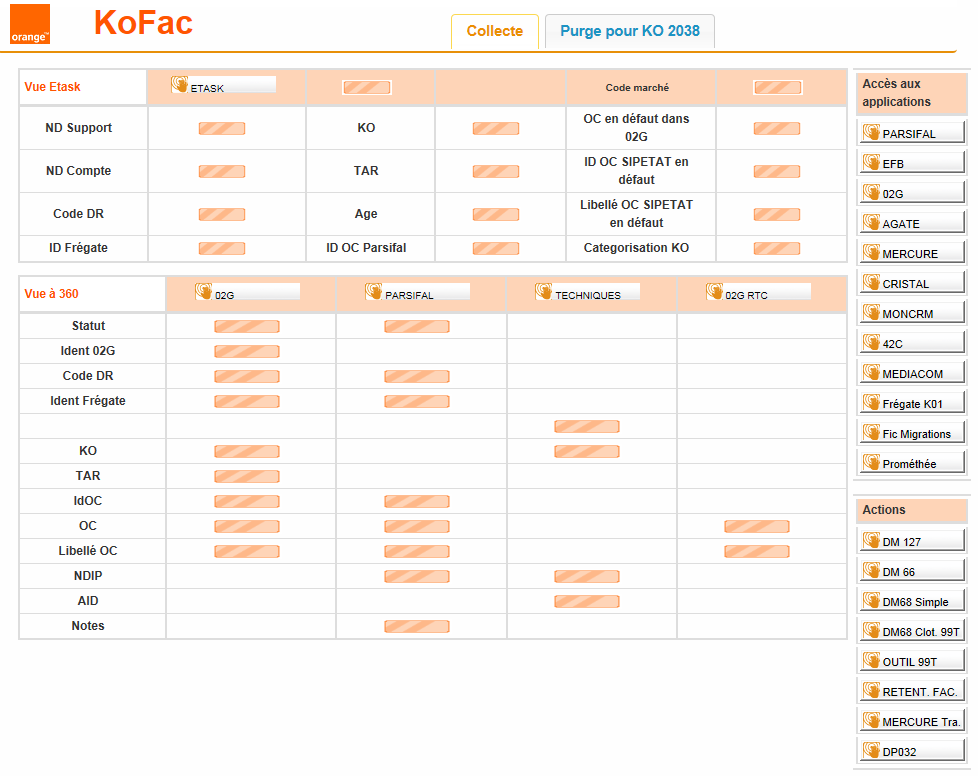
\includegraphics[height=14cm]{Res_KoFac.PNG}\\
\itshape Capture d'écran du résultat de l'application KoFac
\end{center}
\vspace{1cm}
Cette application est utilisée par environ 110 conseillers; le gain de temps attendu est de 12 minutes par dossier pour environ 40 minutes sans Contextor.
\subsection{Les inconvénients}
Pour développer sous Contextor il faut payer des licences développeur mais aussi des licences utilisateurs, ce qui pose problème dans le cas de la réalisation d'un automate destiné à être utilisé par beaucoup d'utilisateurs.
Contextor a aussi un peu de mal à discerner les objets d'une page lorsque celle-ci contient des Iframes.
\subsection{Workflow}
Pendant mon stage une personne travaillant pour Contextor est venu nous présenter les nouveautés liées à l'ajout d'un Workflow dans Contextor. On a donc passé une journée à suivre une présentation des nouveautés de Contextor et plus particulièrement le Workflow. On nous a présenté le Workflow comme quelque chose qui allait nous faire gagner du temps tout en nous permettant d'avoir une meilleure vision du projet. Suite à cela il a été décidé que le prochain projet fait avec Contextor se ferait avec la nouvelle version pour tester l'efficacité du Workflow.
\\\\
\begin{center}
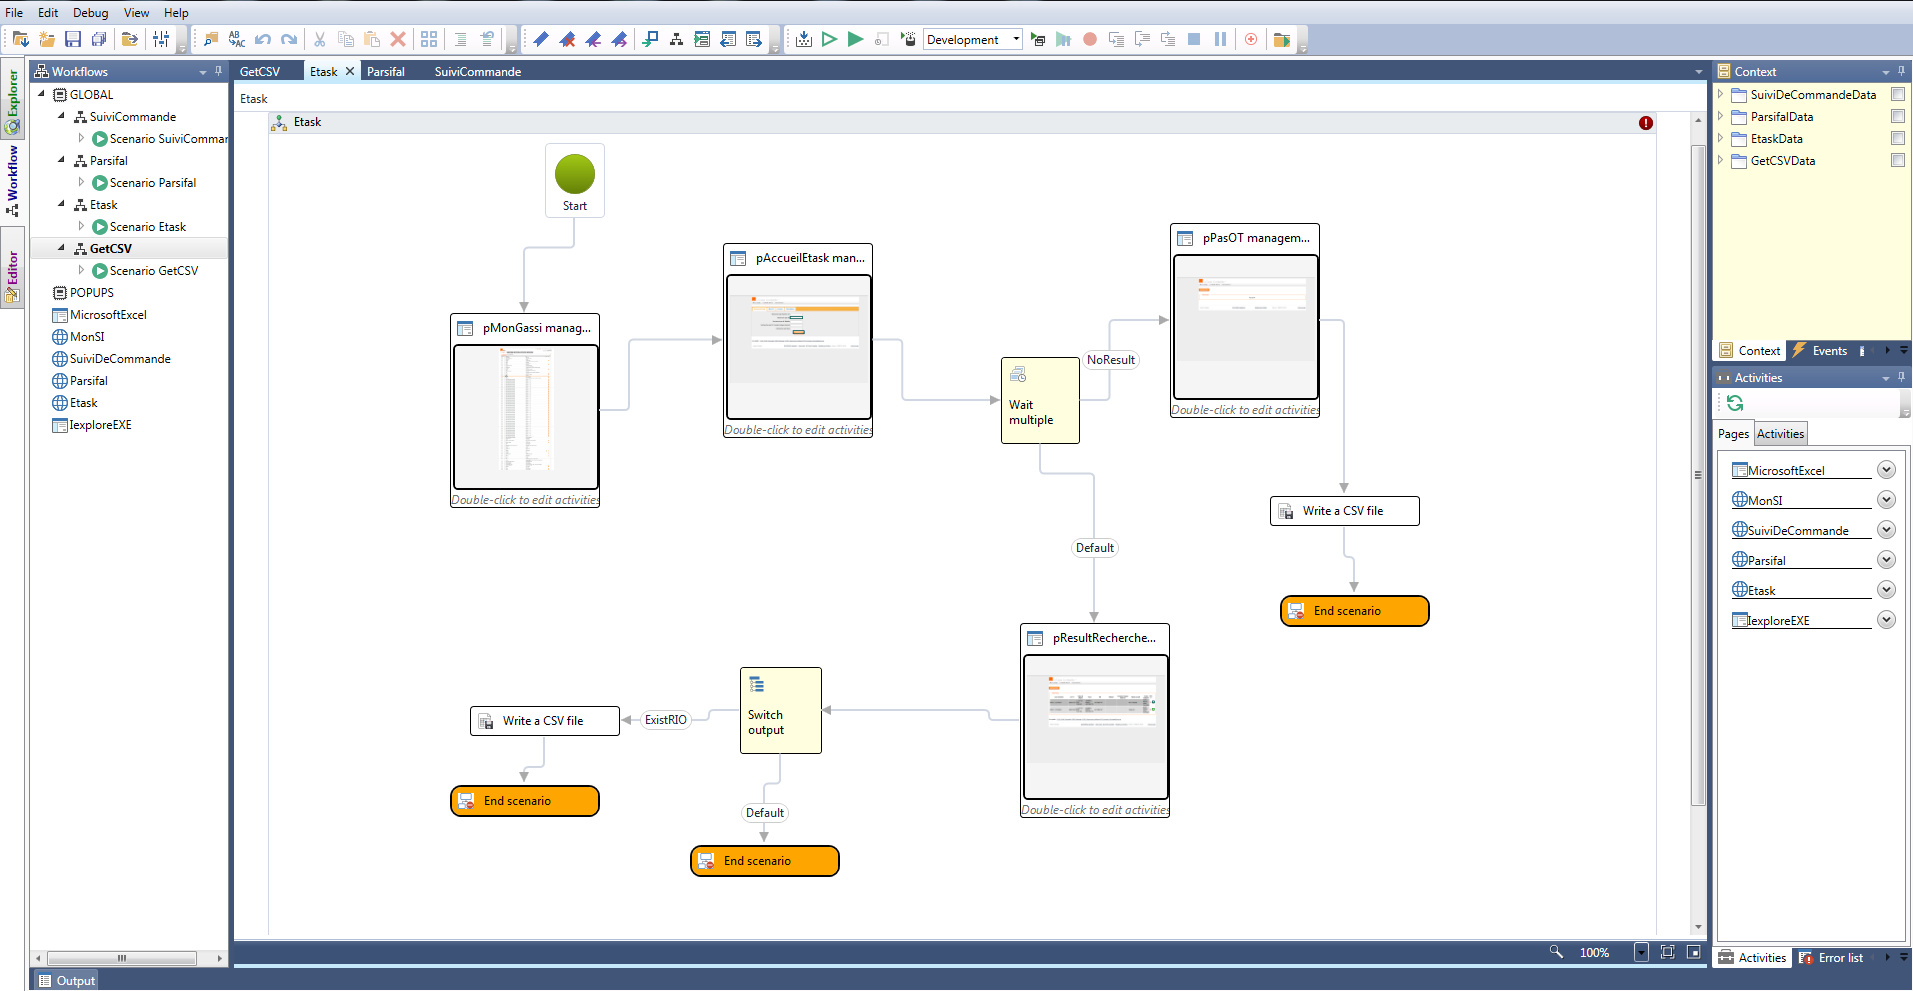
\includegraphics[height=9cm]{workflow2_thibault.PNG}\\
\itshape Capture d'écran du WorkFlow de Contextor pour le projet AutoRio.
\end{center}
\chapter{Missions effectuées}
\section{AutoRio}
\vspace{1cm}
\paragraph {Présentation :}
L'équipe ayant fait la demande pour ce projet reçoit un fichier csv contenant une liste de ND (Numéro de Désignation). Ils doivent alors faire des recherches dans les applications internes à Orange pour trouver des RIO (Relevé d'Identité Opérateur) pour les renseigner dans le fichier csv pour ensuite transmettre ce même fichier à une autre équipe.
\paragraph {Mission :}
Créer un automate qui, à partir des ND présents dans le fichier csv, va parcourir toutes les applications pour trouver des RIO ainsi que vérifier leurs validités à l'aide de règles et ainsi alimenter le fichier csv.\\
\paragraph {Pourquoi cette mission ? :} 
Le temps de travail de l'équipe en charge de remplir le fichier csv de RIO est d'une journée entière par fichier. Or ils reçoivent un fichier tous les jours.\\
Le but était donc leur éviter de passer une journée à faire des tâches répétitives qu'un robot pourrait faire plus rapidement et plus efficacement.
\paragraph {Résolution de la mission :}
Ce projet allait être le projet "Test" pour expérimenter la nouvelle version de Contextor et donc du Workflow.\\
Sur ce projet j'ai travaillé avec Guillaume, un membre de l'équipe.\\
Au début du projet, nous avons élaboré le cahier des charges avec les parties prenantes qui n'étaient pas à l'aise avec ça, pour être sûr de bien comprendre le besoin ainsi que les étapes que le robot devrait suivre.\\
Nous avons utilisé la technique de l'impact mapping qui est une technique de planification stratégique qui permet de ne pas s'égarer durant les phases de développement logiciel. Nous avons donc effectué l'impact mapping sur un mur à l'aide de post-it(\emph{cf annexe C Impact Mapping}).\\
Après avoir réalisé l'impact Mapping, nous avons fait un Workflow en prévision du Workflow que nous devrions faire dans Contextor. Pour ce faire nous avons utilisé un tableau pour pouvoir dessiner notre Workflow(\emph{cf annexe D,E,F Workflow des applications}).\\
Puis lors du début du développement, nous avons commencé à travailler à deux sur le même poste pour apprivoiser le Workflow. Nous devions définir toutes les actions du robot dans le Workflow (ouverture d'application, récupérer la valeur d'un champ, ...) pour qu'ensuite le Workflow nous génère une partie du code avec une base.\\
Une fois cela fait nous avons créé un dépôt sur le git de l'équipe pour pouvoir travailler efficacement.\\
Le robot devait parcourir plusieurs applications. Nous avons donc découpé le projet en plusieurs tâches (Parcours Application 1, Écriture fichier csv, etc)et nous nous sommes partagé les tâches puis nous avons développé les fonctionnalités chacun de notre côté tout en déposant les parties développées sur git et en se tenant informé à la fin de la journée de ce qui a été fait.\\\\
Une fois toutes les fonctionnalités indépendantes développées, nous avons agencé le tout pour que le robot parcourt toutes les applications et remplisse le fichier csv à la fin du traitement.\\
Suite à cela nous avons livré la première version du robot pour que les clients puissent le tester et nous signaler les bugs ainsi que des nouvelles fonctionnalités pour que le robot produise un travail de qualité.
Grâce au retour des clients nous avons perfectionné le robot et il est actuellement utilisé par les clients.\\
Le robot met en moyenne de trente minutes à une heure et demie pour effectuer le traitement, ce qui fait gagner énormément de temps aux clients qui eux avaient besoin d'une journée entière.

\paragraph {Problèmes rencontrés :} 
Lors de ce projet la difficulté rencontrée a été de comprendre le fonctionnement du Workflow car actuellement très peu de documentation est disponible le concernant.\\ Après avoir compris son fonctionnement, nous avons fait face à de nombreux bugs qui ont rendu difficile le développement.\\
Et une fois le robot terminé, lors de l'installation du robot sur les postes des clients, nous nous sommes rendu compte que la nouvelle version de Contextor demandait des versions de Net Framework précises que nous ne pouvions pas installer.\\
Nous avons dû repasser sur l'ancienne version de Contextor tout en modifiant le robot pour qu'il fonctionne sur l'ancienne version. Nous avons donc fait savoir au chef d'équipe que la nouvelle version n'était pas utilisable dans l'état actuel malgré un potentiel énorme.
\newpage
\section{RMM}
\vspace{1cm}
\paragraph {Présentation :}
L'application RMM (Remise de Matériel MultiServices) est une application destinée à la création de commande de matériels de type Livebox, décodeur.\\
Cette application permet de créer uniquement des commandes pour les personnes vivant en Martinique, Guadeloupe, Guyane, Réunion et Mayotte.\\
RMM a été créée à la base pour simplifier l'envoi de matériel dans les îles.\\
L'application est développée sous KitFast en php. 
\paragraph {Mission :} 
Automatiser la création de commande pour les livraisons à domicile à partir d'un fichier csv envoyé quotidiennement par l'application EFB.\\
Et renvoyer un fichier csv contenant toutes les commandes traitées à EFB quotidiennement aussi.
\paragraph {Pourquoi cette mission ? :}
Accélérer la création de commande pour que les commandes soit traitées plus rapidement et par extension que les clients reçoivent plus rapidement leurs produits.
\paragraph {Résolution de la mission :} 
La MOA de l'application RMM est venue dans les locaux de l'équipe une journée pour me présenter le fonctionnement de l'application ainsi que les évolutions que je devrais effectuer sur l'application.\\
Cette journée m'a permis de bien comprendre son fonctionnement ainsi que ce qui était attendu en terme d'évolution.\\
Après avoir compris le fonctionnement de l'application, j'ai schématisé la partie de la base de données que j'allais devoir utiliser pour mener à bien le projet. Cela m'a permis de mieux visualiser le lien entre les tables(\emph{cf annexe G Base de données RMM}).\\
Pendant le développement, j'ai organisé quelques réunions avec la MOA et les membres d'EFB pour discuter de l'avancement du projet, du flux de fichier entre EFB/RMM et pour demander quelques informations supplémentaires.\\
Suite à ça j'ai découpé l'évolution de l'application à faire en plusieurs fonctionnalités, indépendantes, plus petites pour mieux m'organiser et surtout ne rien oublier.\\
Une fois le découpage des tâches fait, j'ai développé les fonctionnalités une par une et les ai testées indépendamment. Une fois toutes les tâches développées et intégrées, j'ai pu faire des tests pour voir si le fonctionnement était le bon.
Suite à ça une fois les tests terminés, j'ai fait une présentation des évolutions de l'application à la MOA sur la Pré-Production.\\
Ensuite la nouvelle version de l'application a été testée par les utilisateurs pour savoir si l'évolution produite satisfaisait les attentes afin d'être passée en Production.
\paragraph {Problèmes rencontrés :}
Le cahier des charges avait été rédigé à la base pour une personne connaissant l'application. Lorsque j'ai reçu ce cahier des charges j'ai été un peu perdu car je ne la connaissais pas du tout.\\
Suite à ça on a organisé la journée décrite plus haut où la MOA est venue me présenter l'application.
\newpage
\section{Aigue Marine}
\vspace{1cm}
\paragraph {Présentation :} 
L'application Aigue Marine est une application déjà existante qui met en relation trois applications, New Agate, Parsifal et Marine. New Agate et Parsifal envoient des données à Aigue Marine qui les traite et les envoie à Marine.\\
\paragraph {Mission :}
Dans ce cas là, il ne s'agit pas d'une grosse évolution de l'application à développer mais plutôt de la maintenance de l'application et de faire des modifications rapides du traitement des fichiers reçus de Parsifal qui est un flux qui a été mis en place récemment.
\paragraph {Résolution de la mission :}
Lors de cette mission, la partie maintenance consiste à, lorsque l'on reçoit un mail disant qu'un problème a été détecté au niveau des fichiers envoyés par Aigue-Marine, retracer le traitement qui a été fait dans Aigue-Marine de la réception des fichiers Parsifal à l'envoi, puis évaluer si le problème vient d'Aigue-Marine ou d'un traitement antérieur à Aigue-Marine. Dans le cas d'une erreur au niveau d'Aigue-Marine, je vais si possible corriger l'erreur, sinon je remonte le problème pour discuter de sa correction.\\
Concernant la partie évolution :\\
Il est arrivé assez souvent que des personnes travaillant du côté de Marine nous demandent de modifier une petite partie du traitement, ce qui a été fait une fois l'évolution demandée. 
\paragraph {Problèmes rencontrés :}
Il n'y a pas eu de réel problème lors de cette mission.\\
En revanche il y a eu quelques petits tracas. Par exemple, au lieu de se concerter de leur côté sur le besoin et de tout nous demander en une seule fois, Marine nous demandait de faire des petites évolutions très souvent (tous les 3-4 jours). Cela nous a fait perdre beaucoup de temps à cause de la partie test du fichier résultant du traitement.
\newpage
\section{Autre}
\vspace{1cm}
\subsection{Lecture d'un RIB}
\vspace{1cm}
\paragraph {Présentation :} 
L'équipe a reçu un projet dont le but était d'automatiser des traitements à partir de données spécifiées sur des RIB au format d'image.
\paragraph {Mission :}
Le but de cette mission était de trouver s'il était possible d'extraire les données d'un RIB peu importe l'inclinaison du RIB sur l'image.
\paragraph {Pourquoi cette mission ? :}
Savoir s'il était possible d'accepter le projet.
\paragraph {Résolution de la mission :}
Lors de cette mission, n'importe quel langage était autorisé pour essayer d'extraire les données d'une image.\\
J'ai donc fait des recherches et je me suis rendu compte que la plupart des personnes utilisait le logiciel Tesseract pour extraire les données d'image.\\
Je l'ai donc téléchargé et testé mais j'ai trouvé deux problèmes majeurs, le premier est qu'une légère inclinaison du RIB fausse totalement l'extraction et le deuxième est que même si le RIB n'est pas incliné, Tesseract fait des erreurs (il confond par exemple les T et les 7).\\
Je n'ai donc trouvé aucun logiciel d'analyse d'image fiable et gratuit (Google en possède un qui marche bien mais qui est payant) et j'en suis arrivé à la conclusion que nous ne pouvions pas prendre le projet.
\paragraph {Problèmes rencontrés :}
Pas de problème majeur, juste un peu ennuyant de faire des recherches et de tomber toujours sur le même logiciel qui ne convient pas à mes attentes.
\newpage
\subsection{Détection d'arrivée de mails}
\vspace{1cm}
\paragraph {Présentation :} 
Le chef de l'équipe CATOP (autre équipe de DevRap) nous a demandé de faire des tests avec Contextor pour voir s'il est capable de détecter la réception de mails possédant des caractéristiques spécifiques (un mot clé dans l'objet par exemple), dans le but d'automatiser un traitement en cas d'arrivée d'un mail.
\paragraph {Mission :}
Vérifier si Contextor est capable de capter les évènements liés à l'arrivée de mails sur Outlook.
\paragraph {Pourquoi cette mission ? :}
Une personne fraudeuse est actuellement en train de commander des dizaines de livebox par mois pour récupérer les codes de livebox qui sont donnés avant la livraison. Après avoir reçu ces codes, il annule les commandes et revend ces codes (je ne sais ce que les acheteurs font de ces codes). Ce que je sais, c'est qu'il faut faire un traitement sur des applications Orange pour bloquer cette personne à chaque fois qu'il est détecté. Et c'est là que le mail intervient. Il faut pouvoir automatiser ce blocage qui peut survenir dans la nuit quand personne n'est présent. 
\paragraph {Résolution de la mission :}
J'ai donc étudié la documentation de Contextor pour voir s'il était possible de faire des choses en rapport avec les mails. J'ai fait un petit programme pour voir si ça marchait bien. J'ai fait des tests et tout fonctionnait comme attendu.\\
J'ai donc confirmé au chef de l'équipe CATOP que c'était possible de faire ce traitement à l'aide de Contextor. Il va sûrement monter un projet si le problème n'a pas été réglé d'une autre manière entre temps.
\paragraph {Problèmes rencontrés :}
La documentation concernant les mails n'étant pas très compréhensible, j'ai dû envoyer des mails à des personnes travaillant chez Contextor pour leur demander des informations concernant la partie mail de Contextor.
\newpage
\chapter{Bilan du stage}
Ce stage m’a permis de découvrir plein de choses tel que l'impact mapping ou même d'appliquer des connaissances vues en cours comme l'utilisation du Kanban.\\\\
J'ai eu la chance de travailler avec une petite équipe très soudée.\\
Chaque membre de l'équipe est toujours disponible pour aider un collègue dans le besoin.\\\\
J’ai constaté qu’il faut toujours poser des questions jusqu'à être sûr d'avoir parfaitement compris l'attendu, être autonome dans son travail et savoir faire des points régulièrement.\\
Mon tuteur et l'ensemble de l'équipe ont su se rendre disponibles pour m'aider et m'accompagner pendant toute la durée du stage.\\
Ceci m'a permis d'être en confiance et de ne pas hésiter à les solliciter.\\\\
La pause repas est l'occasion pour chacun de partager et j'ai pu me rendre compte que cela aide à la cohésion de l'équipe.\\
La petite taille de celle-ci favorise une ambiance sympathique.\\\\
Pour les sujets complexes, j'ai toujours pris le temps d'identifier les différentes étapes que le programme devait réaliser pour effectuer la mission demandée.\\
Ceci me permet de travailler plus efficacement.\\\\
Je suis une personne autonome et cette qualité m'a été utile durant tout le stage.\\
J'avais déjà une bonne méthodologie grâce à l'enseignement universitaire qui m'a été utile.\\\\
Ce stage m'aura permis d'acquérir de nouvelles compétences techniques, de redécouvrir le travail en équipe.
\chapter{Conclusion}
Mon stage dans l’équipe 3MU fut très enrichissant et me conforte dans mon projet professionnel.\\\\
J’ai pu être réintégré dans le monde de l’entreprise dans une équipe de développeurs et découvrir de nouveaux logiciels qui m’étaient inconnus.\\
Je suis heureux d'avoir pu contribuer à l'amélioration du travail des salariés d'Orange, grâce aux différents projets que j'ai réussi à mener à bien.\\\\
Grâce à ce stage je sais à quoi ressemble une méthodologie de projet avec tout ce que ça implique.\\\\
J’ai été très bien accueilli, ce qui a fait de mon stage une très bonne expérience en entreprise.\\\\
Travailler en équipe tout en étant autonome est un aspect qui me plaît beaucoup.\\\\
A l'avenir, ce serait un grand plaisir pour moi de retravailler avec cette équipe.
\newpage
\appendix
\chapter{Direction Orange Île-de-France}
\begin{center}
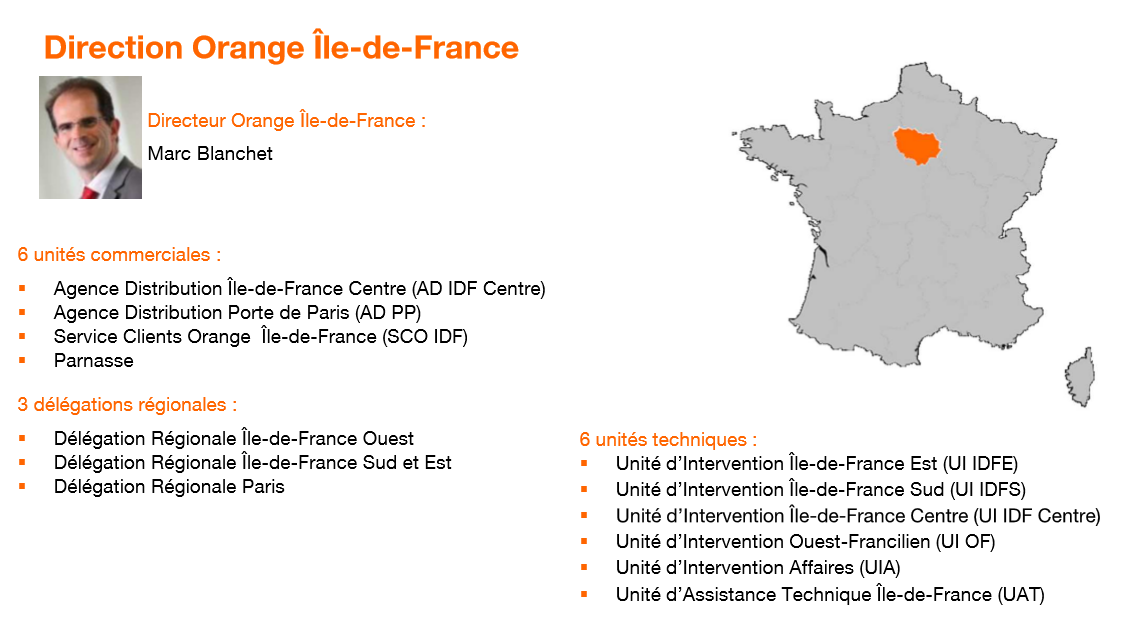
\includegraphics[height=10cm]{direction.PNG}\\
\itshape Schémas des unités de la direction d'orange Île-de-France.
\end{center}
\chapter{Outil de capture de page de Contextor}
\begin{center}
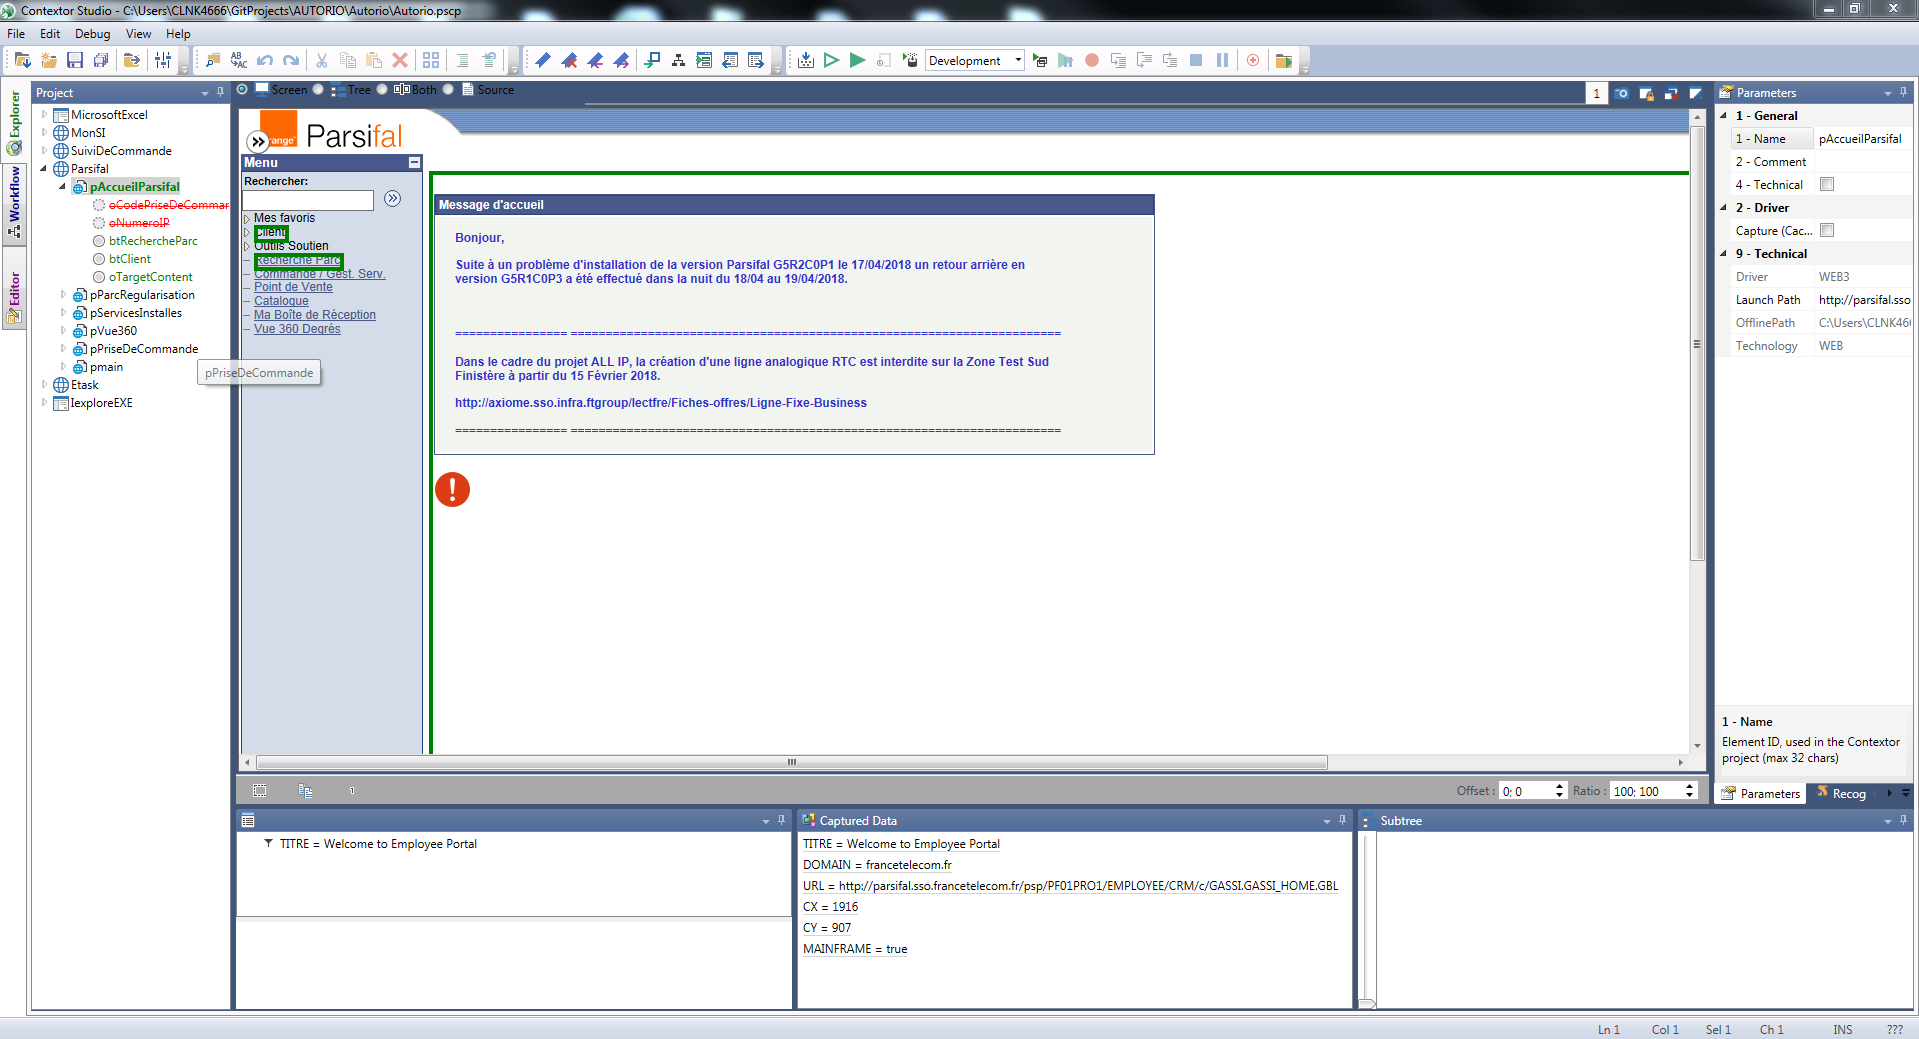
\includegraphics[height=9cm]{contextorCapture.PNG}\\
\itshape Capture d'écran du logiciel Contextor.
\end{center}
Sur l'image, on peut voir la capture de la page d'accueil de l'application Parsifal. On peut observer que certains objets de la page sont encadrés en vert. Il s'agit des objets de la page qui sont stockés dans des variables afin de pouvoir agir sur eux, faire un clic dessus par exemple.
\chapter{Impact Mapping}
\begin{center}
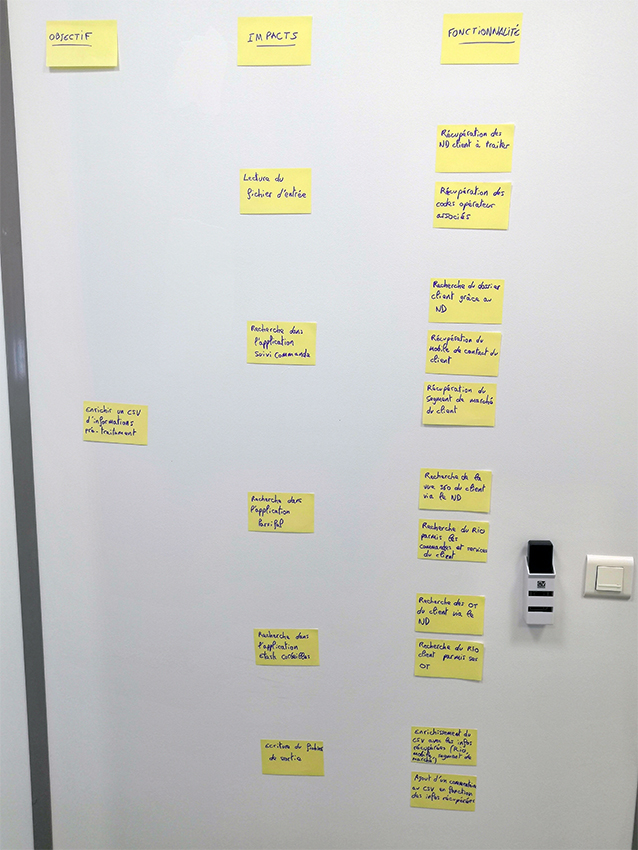
\includegraphics[height=15cm]{impactMappingRIO.jpg}\\
\itshape Photo du résultat de l'impact mapping pour le projet AutoRio.
\end{center}
\chapter{Workflow de l'application SuiviCommande}
\begin{center}
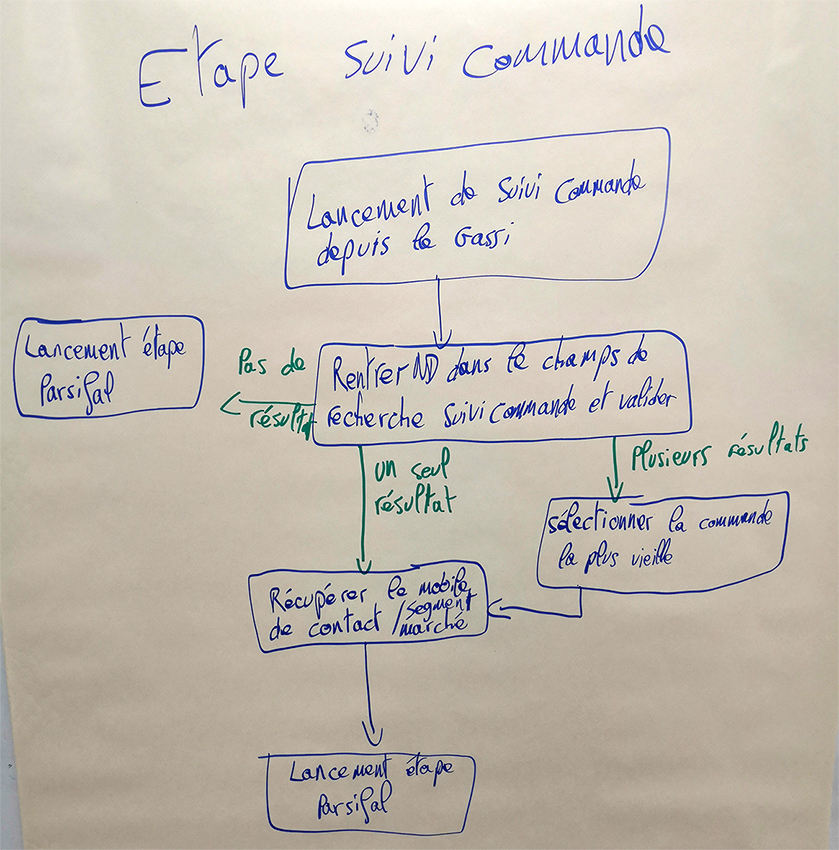
\includegraphics[height=15cm]{workflowSuiviCommande.jpg}\\
\itshape Photo du workflow de l'étape SuiviCommande.
\end{center}
\chapter{Workflow de l'application Parsifal}
\begin{center}
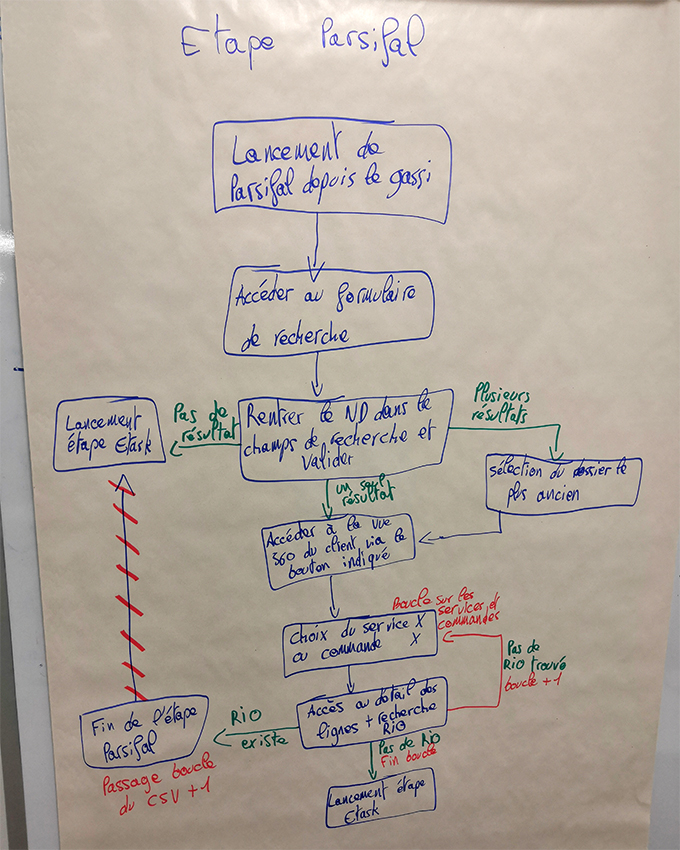
\includegraphics[height=15cm]{workflowParsifal.jpg}\\
\itshape Photo du workflow de l'étape Parsifal.
\end{center}
\chapter{Workflow de l'application Etask}
\begin{center}
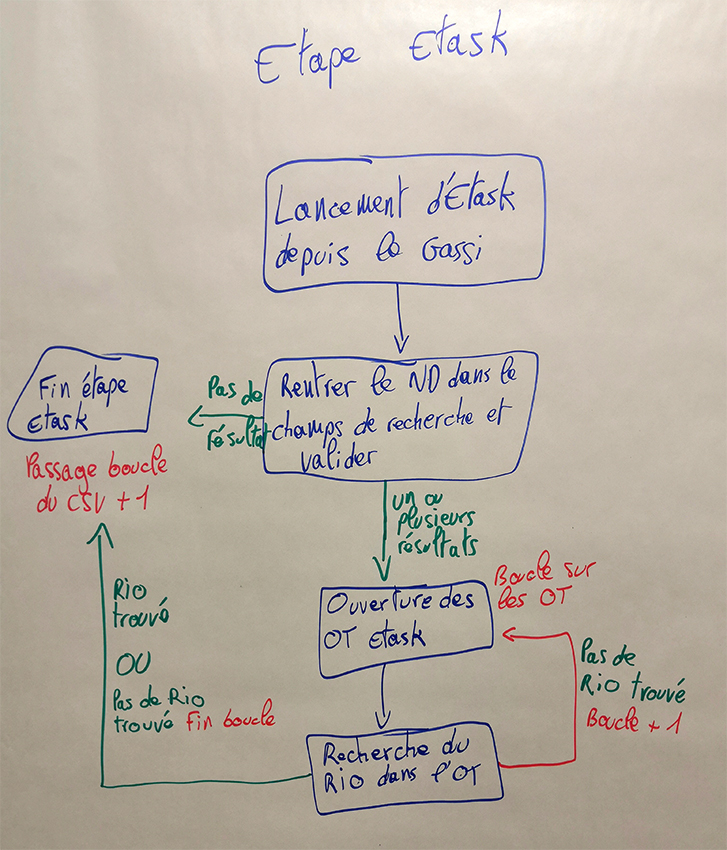
\includegraphics[height=15cm]{workflowEtask.jpg}\\
\itshape Photo du workflow de l'étape Etask.
\end{center}
\chapter{Base de données RMM}
\begin{center}
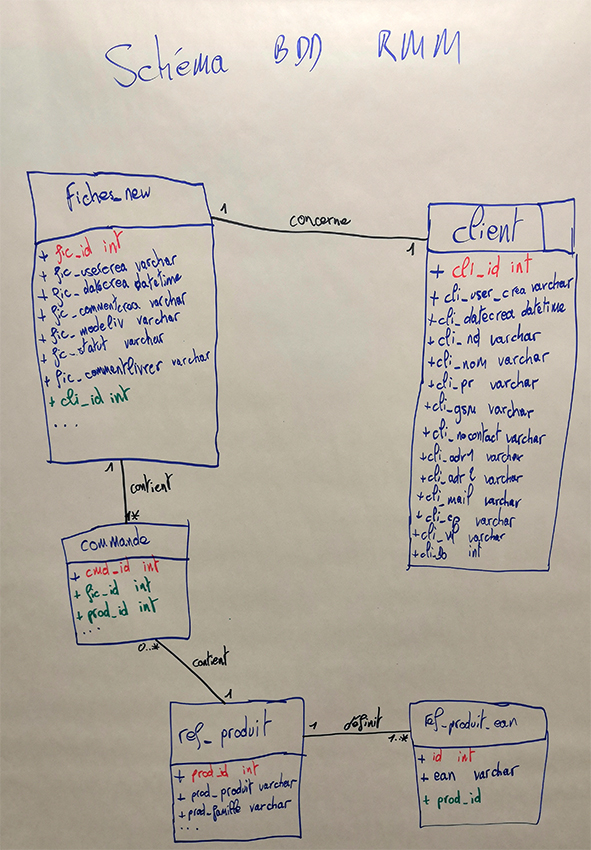
\includegraphics[height=15cm]{schemaBDD_RMM.jpg}\\
\itshape Schéma d'une partie de la base de données de RMM.
\end{center}
\end{document}